\documentclass{article}

% Language setting
\usepackage[brazilian]{babel}
\usepackage[utf8]{inputenc}
\usepackage[T1]{fontenc}

% Set page size and margins
\usepackage[letterpaper,top=2cm,bottom=2cm,left=3cm,right=3cm,marginparwidth=1.75cm]{geometry}

% Useful packages
\usepackage{amsmath}
\usepackage{amsthm}
\usepackage{amssymb}
\usepackage{graphicx}
\usepackage{comment}
\usepackage{amsmath}
\usepackage{xcolor}
\usepackage{float}

\usepackage{parskip}
\usepackage[most]{tcolorbox}
\usepackage[colorlinks=true, allcolors=blue]{hyperref}
\usepackage[brazilian]{cleveref} 

\definecolor{cremeSepia}{RGB}{245, 242, 235}

% Criacao dos ambientes numerados automaticamente no preambulo
\newtcbtheorem[auto counter]{definicao}{Definição}{
	colback=blue!1,
	colframe=blue!75!white,
	fonttitle=\bfseries
}{def}

\newtcbtheorem[auto counter]{teorema}{Teorema}{
	colback=blue!1,
	colframe=blue!75!white,
	fonttitle=\bfseries
}{teo}

\title{VARIATIONAL FORMULATIONS I: Abstract problems.\\
	Computacional}
\author{Victor Matheus da Cunha Santos\\
	NUSP: 13279534}

\begin{document}
	\maketitle
	\pagecolor{cremeSepia}
	
\section*{Problema}	
Given the computational domain $\Omega=\left[0, L_x\right] \times\left[0, L_y\right] \subset \mathbb{R}^2, \partial \Omega=$ $\Gamma_{\text {beft }} \cup \Gamma_{\text {ad }} \cup \Gamma_{\text {right }}$, source term $f$ and thermal diffusivity $\mu$, find temperature field $u$ satisfying

$$
\left\{\begin{array}{rlrl}
	-\nabla \cdot(\mu(\mathbf{x}) \nabla u(\mathbf{x})) & =f(\mathbf{x}) & \mathbf{x} \in \Omega \\
	u(\mathbf{x}) & =u_{\ell} & & \mathbf{x} \in \Gamma_{\text {left }} \\
	u(\mathbf{x}) & =u_r & & \mathbf{x} \in \Gamma_{\text {right }} \\
	-\mu(\mathbf{x}) \nabla u(\mathbf{x}) \cdot \check{\mathbf{n}}(\mathbf{x}) & =0 & & \mathbf{x} \in \Gamma_{\text {ad }}
\end{array}\right.
$$
The thermal diffusivity $\mu$ is piecewise constant and defined by
$$
\mu(\mathbf{x})=\left\{\begin{array}{lll}
	\mu_B & \text { if } & \mathbf{x} \in \Omega_B=\cup_{i=1}^{n_b} \omega_i, \omega_i=\left\{\mathbf{x} \in \Omega,\left\|\mathbf{x}-\mathbf{x}_c^i\right\|<r_i\right\} \\
	\mu_A & \text { if } & \mathbf{x} \in \Omega_A=\Omega \backslash \Omega_B
\end{array}\right.
$$	
	
	
\section{Exercício 1}
	No problema existe dois tipos de condições de contorno e cada uma é aplicada de formas diferentes, as condições de contorno do tipo Neumann são impostas na formulação variacional do problema, quando integramos por partes os termos onde a condição da solução se mostra forte, aparece naturalmente as condições de fronteira do fluxo, e nesse caso podemos aplicar as condições que definem o problema. Já, as condições de Diriclet são impostas no espaço de busca de soluções, nesse caso, escolhemos o espaço de funções contínuas de grau 1, ou seja, funções lineares por partes. A seguir fazemos a formulação variacional e aplicamos as condições de contorno
\subsection*{Formulação Variacional}

\noindent \textbf{Identidade vetorial:}

Para um campo vetorial $\mathbf{F}$ e uma função escalar $v$,
\begin{equation*}
	\nabla\cdot(v\mathbf{F})
	=
	v\,\nabla\cdot\mathbf{F}
	+
	\mathbf{F}\cdot\nabla v.
\end{equation*}

\noindent \textbf{Espaços de funções:}

Definimos o espaço das funções teste por
\begin{equation*}
	V_0
	=
	\left\{
	v\in H^1(\Omega):
	v=0 \text{ em }
	\Gamma_{\mathrm{left}}\cup\Gamma_{\mathrm{right}}
	\right\}.
\end{equation*}

A solução é procurada no conjunto
\begin{equation*}
	V_g
	=
	\left\{
	u\in H^1(\Omega):
	u=u_\ell \text{ em }\Gamma_{\mathrm{left}},
	\quad
	u=u_r \text{ em }\Gamma_{\mathrm{right}}
	\right\},
\end{equation*}
em que as condições de contorno são entendidas no sentido do traço.

\noindent \textbf{Equação integrada:}

Multiplicando a equação de Poisson por uma função teste $v\in V_0$
e integrando sobre o domínio, obtemos
\begin{equation}
	-\int_\Omega
	\nabla\cdot(\mu\nabla u)\,v\,dx
	=
	\int_\Omega fv\,dx.
	\label{eq:poisson-integrada}
\end{equation}

Usando a identidade vetorial com $\mathbf{F}=\mu\nabla u$,
\begin{equation*}
	-v\,\nabla\cdot(\mu\nabla u)
	=
	-\nabla\cdot(v\mu\nabla u)
	+
	\mu\nabla u\cdot\nabla v.
\end{equation*}

Portanto,
\begin{equation*}
	-\int_\Omega
	\nabla\cdot(v\mu\nabla u)\,dx
	+
	\int_\Omega
	\mu\nabla u\cdot\nabla v\,dx
	=
	\int_\Omega fv\,dx.
\end{equation*}

Aplicando o Teorema de Gauss ao termo de divergência,
\begin{equation*}
	\int_\Omega
	\nabla\cdot(v\mu\nabla u)\,dx
	=
	\int_{\partial\Omega}
	\mu\nabla u\cdot\mathbf{n}\,v\,ds,
\end{equation*}
em que $\mathbf{n}$ é a normal unitária exterior ao domínio.

Assim, a integração por partes fornece
\begin{equation*}
	\int_\Omega
	\mu\nabla u\cdot\nabla v\,dx
	-
	\int_{\partial\Omega}
	\mu\nabla u\cdot\mathbf{n}\,v\,ds
	=
	\int_\Omega fv\,dx.
\end{equation*}

Como o contorno é dividido em
\begin{equation*}
	\partial\Omega
	=
	\Gamma_{\mathrm{left}}
	\cup
	\Gamma_{\mathrm{right}}
	\cup
	\Gamma_{\mathrm{ad}},
\end{equation*}
obtemos
\begin{equation*}
	\begin{aligned}
		\int_\Omega \mu\nabla u\cdot\nabla v\,dx
		&-
		\int_{\Gamma_{\mathrm{left}}}
		\mu\nabla u\cdot\mathbf{n}\,v\,ds
		-
		\int_{\Gamma_{\mathrm{right}}}
		\mu\nabla u\cdot\mathbf{n}\,v\,ds
		\\
		&-
		\int_{\Gamma_{\mathrm{ad}}}
		\mu\nabla u\cdot\mathbf{n}\,v\,ds
		=
		\int_\Omega fv\,dx.
	\end{aligned}
\end{equation*}

\noindent \textbf{Aplicação das condições de contorno:}

Nas fronteiras de Dirichlet, os termos de contorno desaparecem porque
\begin{equation*}
	v=0
	\quad\text{em}\quad
	\Gamma_{\mathrm{left}}\cup\Gamma_{\mathrm{right}}.
\end{equation*}

Nas paredes adiabáticas, o termo de contorno desaparece pela condição
de Neumann homogênea:
\begin{equation*}
	-\mu\nabla u\cdot\mathbf{n}=0
	\quad\text{em}\quad
	\Gamma_{\mathrm{ad}}.
\end{equation*}

Consequentemente, a formulação variacional consiste em encontrar
$u\in V_g$ tal que
\begin{equation}
	\underbrace{
		\int_\Omega \mu\nabla u\cdot\nabla v\,dx
	}_{a(u,v)}
	=
	\underbrace{
		\int_\Omega fv\,dx
	}_{\ell(v)}
	\qquad\forall v\in V_0.
	\label{eq:poisson-variacional}
\end{equation}

As condições de Dirichlet são incorporadas ao conjunto de busca
$V_g$. A condição adiabática é incorporada naturalmente à formulação
variacional pela anulação do termo de fluxo nas paredes superior
e inferior.

Para $\mu$ descontínuo nas interfaces das inclusões, a integração
por partes pode ser realizada em cada região. Na derivação a partir
de uma solução suficientemente regular por partes, as contribuições
das interfaces se cancelam pela continuidade do fluxo normal e
pelo uso de funções teste de $H^1(\Omega)$.



\vspace{1cm}
\noindent \textbf{Formas discretas:}
\begin{align*}
	a &= \text{inner}(\text{mu} \ast \text{grad}(u), \text{grad}(v)) \, dx \\
	l &= f \, v \, dx
\end{align*}

\subsection*{Fluxo Zero}
O fluxo zero é importa nas paredes, de cima e de baixo, é uma condição do tipo Neumann que indicam a ausência de fluxo normal de calor, nesse caso ela é aplicada nas paredes
\[
\mu(x) \nabla u(x) \cdot \hat{n} = 0
\]

\noindent \textbf{}
\begin{figure}[H]
	\centering
	\caption[Esquema visual dos elementos e faces]{}
	\label{fig:boundaries}
	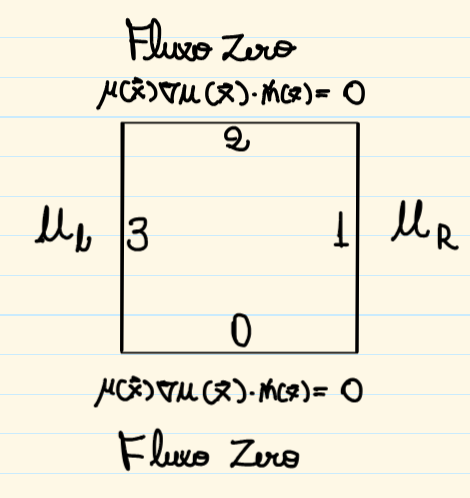
\includegraphics[width=0.4\linewidth]{boundaries}
\end{figure}


\noindent \textbf{Onde entra $u_l$ e $u_r$?}

\noindent É criado uma tag para cada parede.
\[
\text{bcs} = \{ (V_h, \text{u\_left}, 3), (V_h, \text{u\_right}, 1) \}
\]

\section{Exercício 2}


\begin{figure}[H]
	\centering
	\caption{}
	\label{fig:meshsurface}
	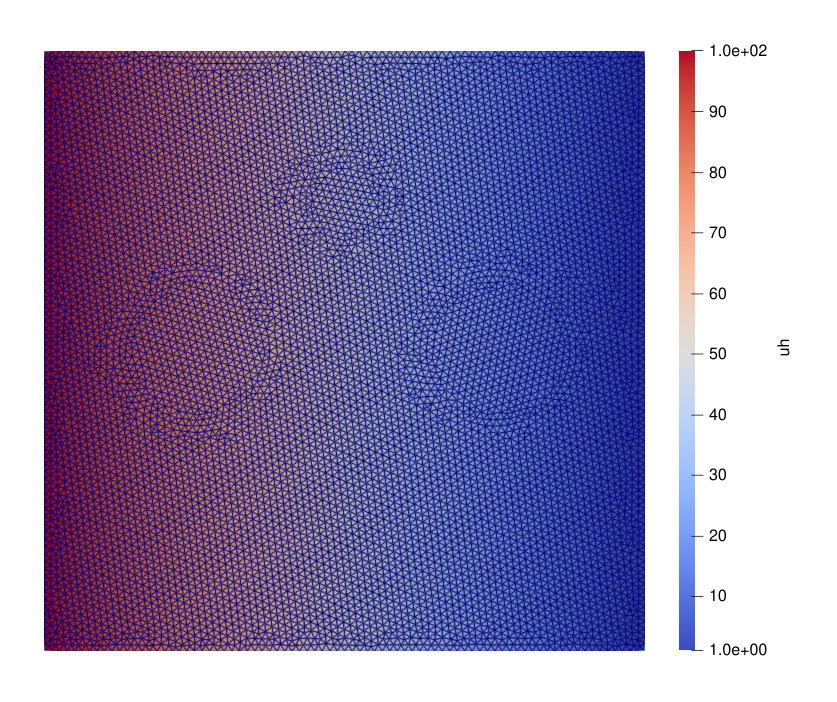
\includegraphics[width=0.4\linewidth]{mesh_surface}
\end{figure}


\section{Exercício 3 - 4}
\subsection{Normas}
\begin{equation}
	\|u - u_{h}\|_{H^{1}} = \left( \int_{\Omega} (u - u_{h})^{2} + \| \nabla(u - u_{h}) \|^{2} dx  \right) ^{1/2}
\end{equation}

\begin{equation}
	\|u - u_{h}\|_{L^{2}} = \left( \int_{\Omega} (u - u_{h})^{2} dx  \right) ^{1/2}
\end{equation}
\subsection{Comparação entre situações}
Com a situação que temos fonte nula e condições de Dirichlet não-homogêneas ($u_l = 100, ~ u_r = 1$ e $f = 0$), para a seguinte solução analítica: 

\begin{equation}
	u_e(\mathbf{x}) = u_{\ell} - \frac{u_{\ell} - u_r}{L_x} x
\end{equation}

\begin{figure}[H]
	\centering
	\caption{}
	\label{fig:perfiltransversaluh}
	\includegraphics[width=0.4\linewidth]{figures/perfil_transversal_uh_uexata}
\end{figure}

\begin{table}[H]
	\centering
	\caption{Erros de aproximação}
	\label{tab:erros}
	\begin{tabular}{lc}
		\hline
		\textbf{Erro} & \textbf{Valor} \\
		\hline
		$L^2$ error & $1.114 \times 10^{-12}$ \\
		$H^1$ error & $4.267 \times 10^{-12}$ \\
		\hline
	\end{tabular}
\end{table}
Com a situação em que temos fonte não nula e condições de Dirichlet homogêneas ($u_l = 0, ~ u_r = 0$ e $f = 100$), para a seguinte solução analítica: 

\begin{equation}
	u_e(\mathbf{x}) = 50*x(L_x - x).
\end{equation}

\begin{figure}[H]
	\centering
	\caption{}
	\label{fig:perfiltransversal_f100}
	\includegraphics[width=0.4\linewidth]{figures/perfil_transversal_uh_uexata_f100}
\end{figure}

\begin{table}[htbp]
	\centering
	\caption{Error norms since analytical solution is available ($\mu_A=\mu_B$ and $f=0$)}
	\label{tab:error-norms}
	\begin{tabular}{lc}
		\hline
		\textbf{Error} & \textbf{Value} \\
		\hline
		$L^2$ error & $0.008521501512041887$ \\
		$H^1$ error & $1.2456604608567208$ \\
		\hline
	\end{tabular}
\end{table}

Quando estudamos o erro entre \(u\) e \(u_h\), quando \(u\) é uma função linear, verifica-se que o espaço de funções ao qual \(u_h\) pertence (CG1), ou seja, funções lineares contínuas e de grau um, representa exatamente as características de \(u\). Além disso, \(u'\) é constante e \(u_h'\) também é constante; nessa situação a escolha do espaço é adequada. Por outro lado, quando \(u\) é uma função quadrática, o CG1 torna-se um espaço de funções menos adequado, visto que \(u'\) agora é linear enquanto que \(u_h'\) é constante, comparando graficamente,


\begin{figure}[H]
	\centering
	\caption{}
	\label{fig:erro_interpret}
	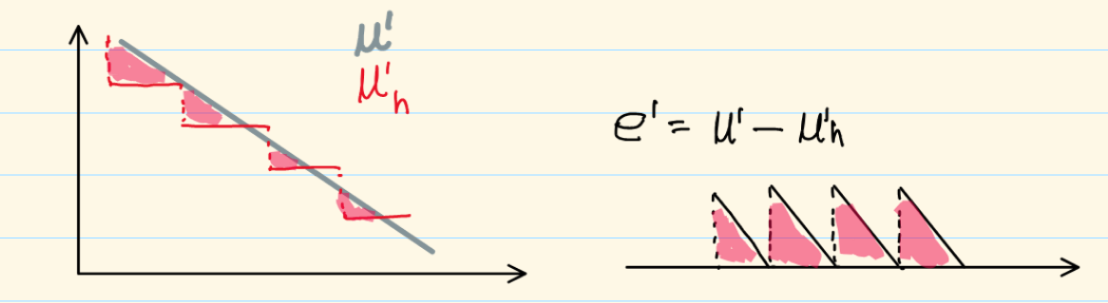
\includegraphics[width=0.6\linewidth]{figures/erros_interpret}
\end{figure}

Além do que ocorre com \(u'\) e \(u_h'\), no caso em que \(u\) é quadrática e \(u_h\) está em CG1,

\begin{figure}[H]
	\centering
	\caption{}
	\label{fig:erro_quadratica}
	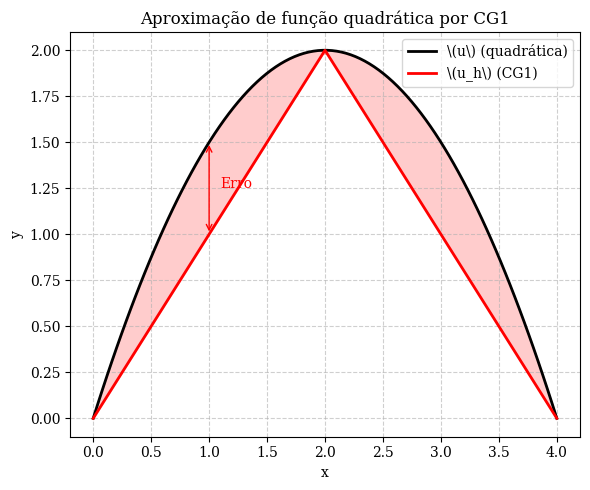
\includegraphics[width=0.4\linewidth]{figures/cg1_quadratica}
\end{figure}


De fato, a norma \(H^1(\Omega)\) é mais adequada para enxergar o que acontece com \(u'\) e \(u_h'\).


\begin{comment}
	

\begin{figure}[H]
	\centering
	\begin{minipage}{0.48\linewidth}
		\centering
		\caption{}
		\label{fig:ueuh}
		\includegraphics[width=\linewidth]{ue_uh}
	\end{minipage}
	\hfill
	\begin{minipage}{0.48\linewidth}
		\centering
		\caption{}
		\label{fig:ueuh_f100}
		\includegraphics[width=\linewidth]{ue_uh_f100}
	\end{minipage}
\end{figure}
\end{comment}

\section{Exercício 7}
Na primeira situação fonte nula e condições de Dirichlet não homogêneas  ($u_l = 100,  u_r = 1$ e $f = 0$) , calculamos a difusividade termal efetiva, 

\begin{equation}
	\mu_{eff} = \frac{|Q| / L_{y}}{|u_{l} - u_{r}|/L_{x}}
\end{equation}

\begin{table}[htbp]
	\centering
	\caption{Resultados da simulação}
	\label{tab:resultados_nonhomogen}
	\begin{tabular}{lc}
		\hline
		\textbf{Grandeza} & \textbf{Valor} \\
		\hline
		$Q_{in}$ & $99.00$ \\
		$Q_{out}$ & $98.99$ \\
		Power & $0.0$ \\
		Resíduo do balanço & $-3.282 \times 10^{-12}$ \\
		$\mu_{eff}$ & $0.999$ \\
		\hline
	\end{tabular}
\end{table}
Verifca-se pela \cref{tab:resultados_nonhomogen} que com o resultado que, quando ($\mu_{A} = \mu_{B} = 1$) o \(\mu_{eff}\) recupera esse valor, fisicamente podemos dizer que o domínio é um único material. 
O coeficiente \(\mu\) relaciona a variação da temperatura($\nabla u$) ao fluxo de calor $\mathbf q$:
\begin{equation*}
	\mathbf q=-\mu\nabla u.
\end{equation*}
Isso significa que, para o mesmo gradiente de temperatura, um material com maior \(\mu\) permite um fluxo maior de calor. O produto do $\mu$ com o ($\nabla u$) representa um escalar multiplicando um campo vetorial, o que faz a magnitude dos vetores resultando modificar, nesse caso o fluxo do calor aumenta ou diminuir dependendo de $\mu$. O sinal negativo indica que o calor flui da região mais quente para a mais fria.
Para um material homogêneo, a temperatura varia linearmente, e o módulo do gradiente é
\begin{equation*}
	|\nabla u|=\frac{|u_\ell-u_r|}{L_x}.
\end{equation*}
Assim, o fluxo por unidade de área é
\begin{equation*}
	|q_x|=\mu\frac{|u_\ell-u_r|}{L_x}.
\end{equation*}
Como \(Q\) é o fluxo integrado sobre a lateral de comprimento \(L_y\), temos \(|Q|/L_y=|q_x|\), na interpretação bidimensional por unidade de espessura. Isolando o coeficiente:
\begin{equation*}
	\mu_{\mathrm{eff}}
	\frac{|Q|/L_y}{|u_\ell-u_r|/L_x}.
\end{equation*}


\section{Exercício 8}
\begin{table}[H]
	\centering
	\caption{Resultados da simulação}
	\label{tab:resultados_exe8}
	\begin{tabular}{lc}
		\hline
		\textbf{Grandeza} & \textbf{Valor} \\
		\hline
		$Q_{in}$ & $-197.89$ \\
		$Q_{out}$ & $197.81$ \\
		Power & $400.00$ \\
		$ - Q_{in} + Q_{out}$ & $395.70$ \\
		Resíduo do balanço & $-4.2900$ \\
		\hline
	\end{tabular}
\end{table}


\section{Exercício 9}
Com os seguintes parâmetros,\(\mu_A=5\), \(\mu_B=500\), \(f=100\), \(u_\ell=u_r=0\)
\begin{figure}[H]
	\centering
	\caption{}
	\label{fig:exe9}
	\includegraphics[width=0.4\linewidth]{figures/exe_9}
\end{figure}

\section{Exercício 10}
\begin{equation*}
	E_i(h)
	\left|
	\overline T_i^h-\overline T_i^{\mathrm{ref}}
	\right|.
\end{equation*}


\begin{figure}[H]
	\centering
	\caption{}
	\label{fig:exe10}
	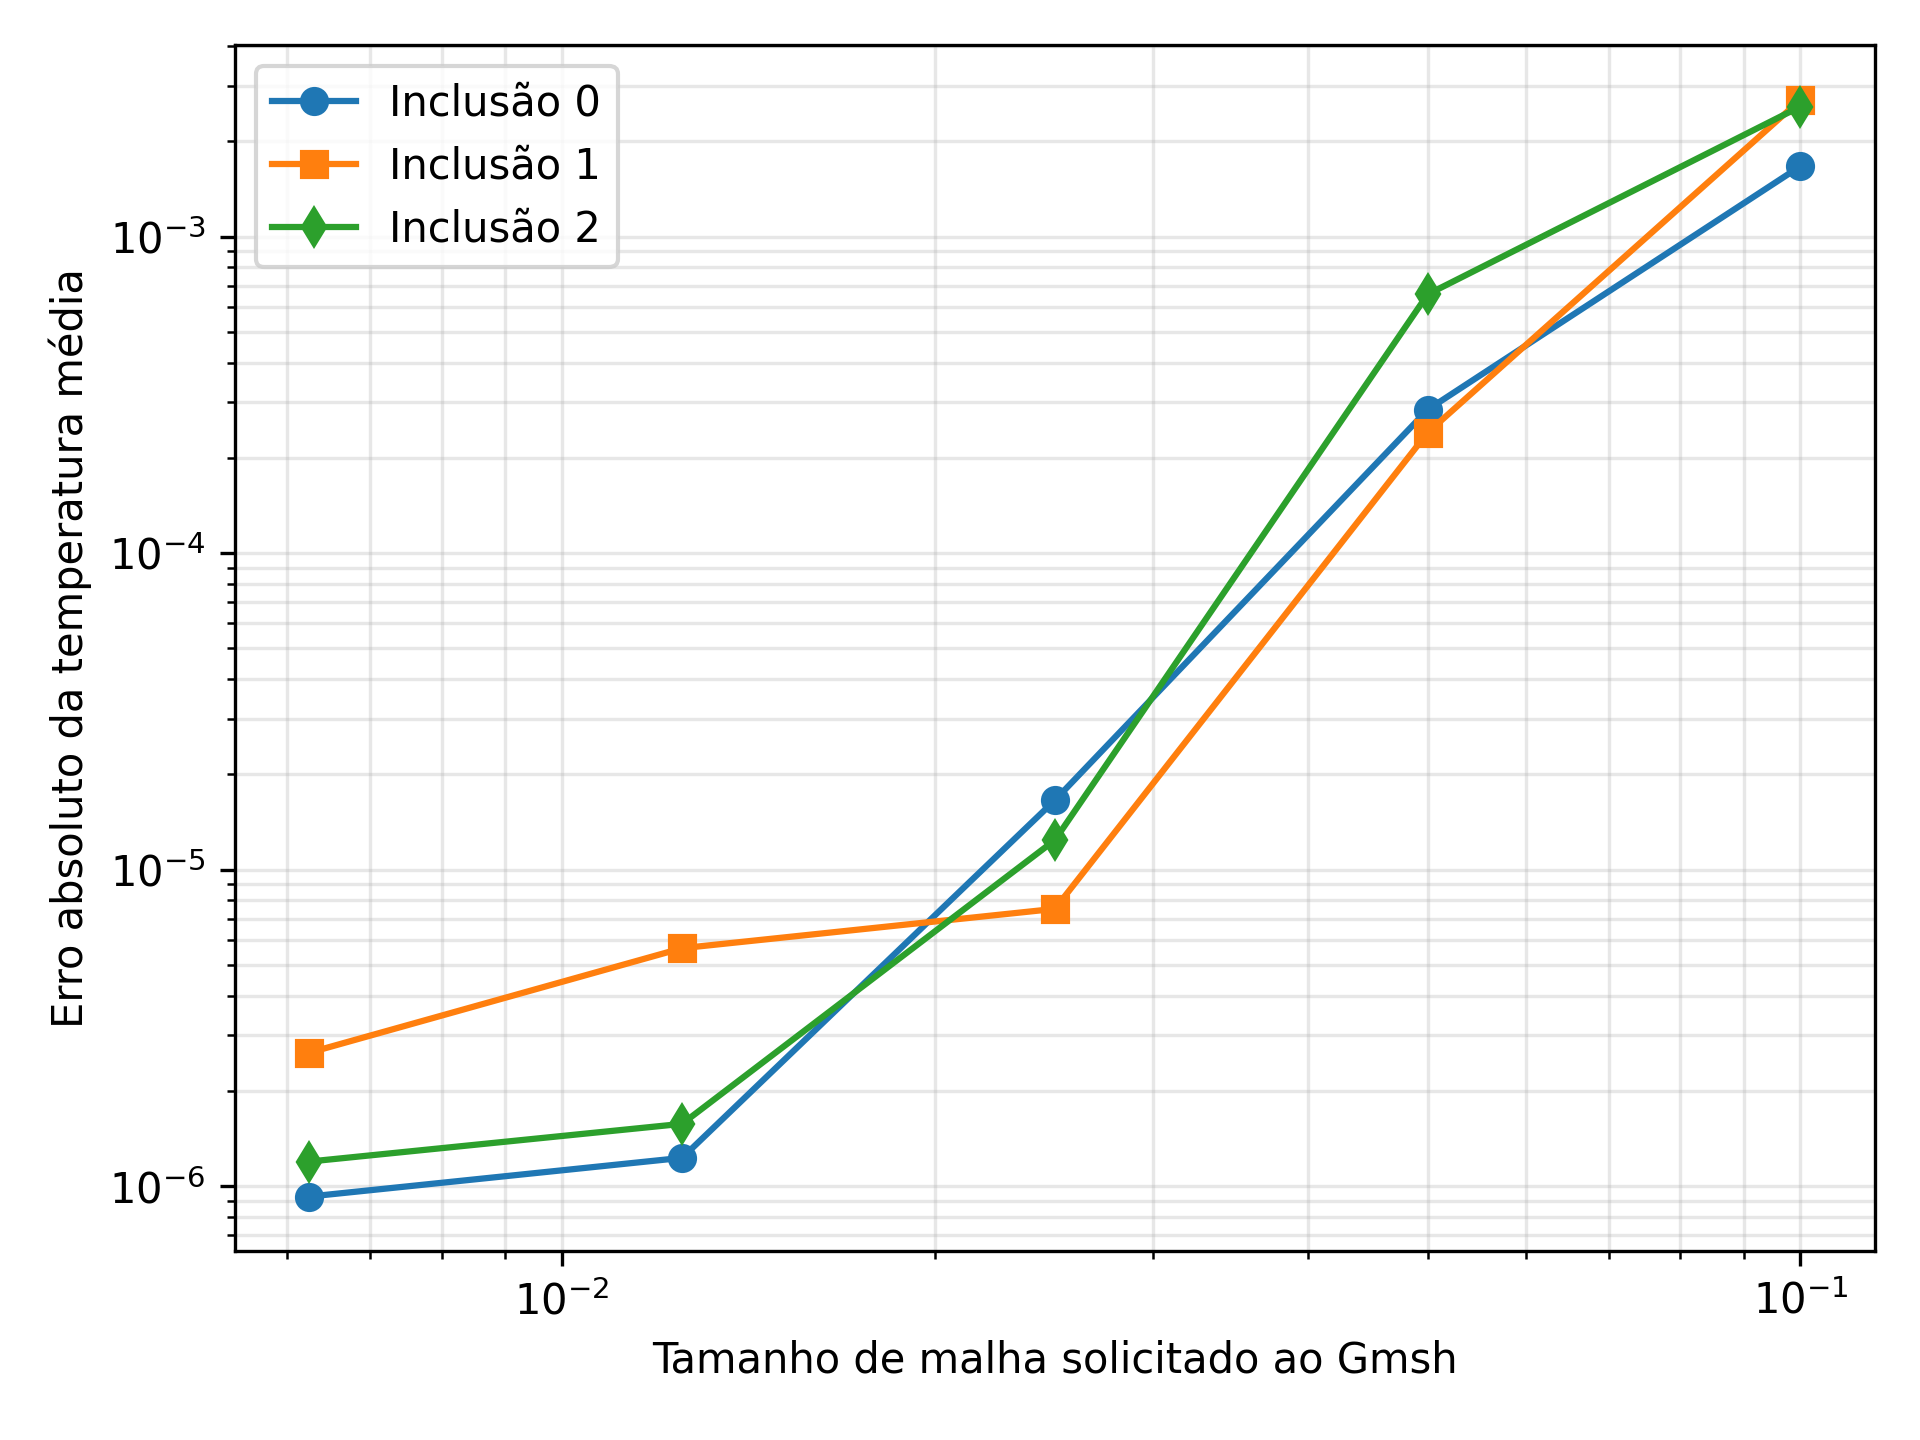
\includegraphics[width=0.4\linewidth]{figures/converg}
\end{figure}
\begin{table}[H]
	\centering
	\caption{Temperaturas médias nas inclusões e erros absolutos em relação à malha de referência. A coluna ``Elementos'' apresenta a contagem total
		reportada pelo gerador de malhas.}
	\label{tab:medias-inclusoes}
	\begin{tabular}{ccccccccc}
		\hline
		$h$ & Nós & Elementos & $T_0$ & $T_1$ & $T_2$ & $E_0$ & $E_1$ & $E_2$ \\
		\hline
		0.10000 & 565     & 1.177   & 6.098348 & 8.115329 & 6.097441 & $1.67\times10^{-3}$ & $2.70\times10^{-3}$ & $2.58\times10^{-3}$ \\
		0.05000 & 2.054   & 4.196   & 6.099733 & 8.117793 & 6.099360 & $2.84\times10^{-4}$ & $2.40\times10^{-4}$ & $6.57\times10^{-4}$ \\
		0.02500 & 7.738   & 15.645  & 6.100000 & 8.118040 & 6.100029 & $1.66\times10^{-5}$ & $7.52\times10^{-6}$ & $1.24\times10^{-5}$ \\
		0.01250 & 30.302  & 60.937  & 6.100018 & 8.118039 & 6.100018 & $1.23\times10^{-6}$ & $5.65\times10^{-6}$ & $1.58\times10^{-6}$ \\
		0.00625 & 119.756 & 240.172 & 6.100018 & 8.118036 & 6.100018 & $9.28\times10^{-7}$ & $2.64\times10^{-6}$ & $1.20\times10^{-6}$ \\
		0.00313 & 475.831 & 952.975 & 6.100017 & 8.118033 & 6.100017 & --- & --- & --- \\
		\hline
	\end{tabular}
\end{table}
Podemos verificar que os erros das três temperaturas médias diminuem com o refinamento, mesmo que as taxas de redução variem entre as malhas. As médias próximas de \(6{,}100017\), \(8{,}118033\) e \(6{,}100017\) indicam estabilização desses valores em relação à referência utilizada que foi $h_{\mathrm{ref}}=0.003125$ e 475\,831 nós.
\end{document}